% Original book diagram: fig:bayes_thm
% Book source: sections/Part_I/bayes_theorem.tex
% Original diagram authorship retained. Visual design: Ziad Mosalam.
\documentclass[11pt,border=8pt]{standalone}
\usepackage{amsmath,amssymb,graphicx,tikz}
\usetikzlibrary{arrows.meta,automata,positioning,calc,shapes.geometric,fit,backgrounds,patterns}
\newcommand{\vect}[1]{\mathbf{#1}}
\newcommand{\mat}[1]{\mathbf{#1}}
\newcommand{\Normal}{\mathcal{N}}
\newcommand{\prob}{p}
\newcommand{\E}{\mathbb{E}}
\newcommand{\Var}{\mathrm{Var}}
\newcommand{\Cov}{\mathrm{Cov}}
\newcommand{\CovP}{\mathbf{P}}
\newcommand{\Prob}{\mathbb{P}}
\setlength{\textwidth}{6.5in}
% Shared visual vocabulary for the book's original diagrams.
% Figures opt in explicitly, so unrelated text and existing additions are unchanged.
\definecolor{BookBlue}{HTML}{003262}
\definecolor{BookGold}{HTML}{B17A00}
\definecolor{BookTeal}{HTML}{247C86}
\definecolor{BookInk}{HTML}{30363B}
\definecolor{BookLight}{HTML}{E9EFF5}
\tikzset{
  book figure/.style={font=\small\rmfamily, color=BookBlue, text=BookInk,
    line width=0.8pt, >=Latex},
  book axis/.style={->, draw=BookInk, line width=0.6pt},
  book link/.style={->, draw=BookBlue, line width=0.8pt},
  book observation/.style={draw=BookGold, fill=BookGold!8},
  book state/.style={draw=BookBlue, fill=BookLight},
  book note/.style={font=\footnotesize\rmfamily, text=BookInk}
}

\begin{document}
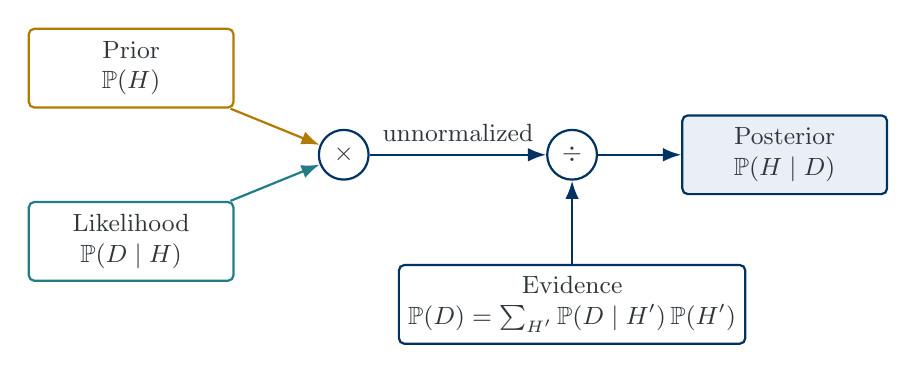
\begin{tikzpicture}[font=\small, text=BookInk, draw=BookBlue, line width=0.8pt, >=Latex, every node/.style={font=\small},
box/.style={draw=BookBlue, fill=white, rectangle, rounded corners=2pt, align=center, minimum width=2.6cm, minimum height=1cm}]
\node[box,draw=BookGold] (prior) at (0,1.1) {Prior\\$\Prob(H)$};
\node[box,draw=BookTeal] (lik) at (0,-1.1) {Likelihood\\$\Prob(D\mid H)$};
\node[draw=BookBlue, fill=white, circle, inner sep=3pt] (prod) at (2.7,0) {$\times$};
\node[draw=BookBlue, fill=white, circle, inner sep=3pt] (div) at (5.6,0) {$\div$};
\node[box,fill=BookLight] (post) at (8.3,0) {Posterior\\$\Prob(H\mid D)$};
\node[box] (ev) at (5.6,-1.9) {Evidence\\$\Prob(D)=\sum_{H'}\Prob(D\mid H')\,\Prob(H')$};
\draw[->, draw=BookGold, line width=0.8pt] (prior) -- (prod);
\draw[->, draw=BookTeal, line width=0.8pt] (lik) -- (prod);
\draw[->, line width=0.8pt] (prod) -- node[above=1pt]{\small unnormalized} (div);
\draw[->, line width=0.8pt] (ev) -- (div);
\draw[->, line width=0.8pt] (div) -- (post);
\end{tikzpicture}
\end{document}
